% ==============================================================================
% CHƯƠNG 3: PHƯƠNG PHÁP THỰC HIỆN
% ==============================================================================

\chapter{PHƯƠNG PHÁP THỰC HIỆN}
\label{chap:methodology}

Chương này trình bày chi tiết phương pháp tiếp cận và thiết kế hệ thống. Thay vì chỉ mô tả \textit{làm gì}, chúng tôi cố gắng trả lời \textit{tại sao} --- giải thích lý do đằng sau mỗi quyết định thiết kế, từ góc nhìn của một nhà nghiên cứu muốn hiểu sâu bản chất vấn đề.

\section{Tổng quan kiến trúc hệ thống}

\subsection{Triết lý thiết kế}

Hệ thống phân loại chất lượng chuối được thiết kế theo kiến trúc \textbf{2 giai đoạn} (two-stage pipeline), kết hợp điểm mạnh của object detection và image classification. Lựa chọn này không chỉ xuất phát từ yêu cầu kỹ thuật mà còn từ nhận thức sâu sắc về bản chất dữ liệu: hầu hết các tập dữ liệu công khai về độ chín chuối đều là classification datasets (folder-per-class, không có bounding box), trong khi giao diện người dùng lại yêu cầu hiển thị vị trí của chuối trong khung hình.

\textbf{Quyết định thiết kế cốt lõi:}

\begin{enumerate}
    \item \textbf{Constraints dẫn dắt thiết kế, không phải ngược lại}: Việc không có bounding box annotation trong Kaggle dataset là một constraint, nhưng thay vì coi đó là hạn chế, chúng tôi biến nó thành cơ hội để tận dụng COCO pretrained detector --- một mô hình đã được huấn luyện trên hàng triệu ảnh.
    
    \item \textbf{Separation of concerns}: Detector lo việc \textit{đâu là chuối}, classifier lo việc \textit{chuối này chất lượng thế nào}. Mỗi component có thể được cải tiến độc lập mà không ảnh hưởng đến component khác.
    
    \item \textbf{Transfer learning như là lợi thế cạnh tranh}: Với nguồn lực hạn chế của một dự án học thuật, việc kế thừa tri thức từ các mô hình pretrained là chiến lược thông minh hơn việc cố gắng train from scratch.
\end{enumerate}

\begin{figure}[H]
\centering
\begin{tikzpicture}[
    node distance=1.5cm,
    block/.style={rectangle, draw, fill=blue!20, text width=3cm, text centered, rounded corners, minimum height=1.2cm},
    decision/.style={diamond, draw, fill=yellow!20, text width=2.5cm, text centered, aspect=2},
    arrow/.style={->, thick}
]
    % Input
    \node[block, fill=green!30] (input) {Video Frame\\(Webcam)};
    
    % Detector
    \node[block, below of=input] (detector) {YOLO Detector\\(COCO pretrained)};
    
    % Decision
    \node[decision, below of=detector, yshift=-0.5cm] (check) {Tìm thấy\\chuối?};
    
    % Classifier
    \node[block, below of=check, yshift=-0.5cm] (classifier) {YOLO Classifier\\(Fine-tuned)};
    
    % Analyzer
    \node[block, right of=classifier, xshift=3cm] (analyzer) {Banana Analyzer\\(Feature Extraction)};
    
    % Aggregator
    \node[block, below of=classifier] (aggregator) {Result Aggregator\\(Multi-bbox)};
    
    % Output
    \node[block, below of=aggregator, fill=red!30] (output) {UI Display\\(Grading Result)};
    
    % No detection path
    \node[block, right of=check, xshift=3cm, fill=gray!30] (nodetect) {Không phát hiện\\(Hold bbox)};
    
    % Arrows
    \draw[arrow] (input) -- (detector);
    \draw[arrow] (detector) -- (check);
    \draw[arrow] (check) -- node[left] {Có} (classifier);
    \draw[arrow] (check) -- node[above] {Không} (nodetect);
    \draw[arrow] (nodetect) |- (aggregator);
    \draw[arrow] (classifier) -- (analyzer);
    \draw[arrow] (classifier) -- (aggregator);
    \draw[arrow] (analyzer) -- (aggregator);
    \draw[arrow] (aggregator) -- (output);
\end{tikzpicture}
\caption{Kiến trúc tổng quan hệ thống phân loại chất lượng chuối}
\label{fig:system_architecture}
\end{figure}

\section{Pipeline xử lý 2 giai đoạn}

\subsection{Giai đoạn 1: Object Detection}

Mục tiêu của giai đoạn này là xác định \textbf{vị trí} của tất cả quả chuối trong khung hình. Chúng tôi sử dụng YOLOv8n pretrained trên COCO dataset, trong đó class ``banana'' đã được định nghĩa sẵn (class ID = 46 trong COCO).

\textbf{Lý do không train detector riêng từ đầu:}
\begin{enumerate}
    \item \textbf{COCO detector đã đủ tốt cho việc định vị chuối trong điều kiện bình thường}. COCO dataset bao gồm 80 class, trong đó ``banana'' (class ID 46) đã được train trên hàng ngàn ảnh đa dạng.
    
    \item \textbf{Tiết kiệm công sức label bounding box} --- một công việc tốn thời gian và dễ sai sót. Với dataset 13,500 ảnh, việc vẽ bounding box thủ công sẽ tiêu tốn vài tuần làm việc.
    
    \item \textbf{Tập trung nguồn lực vào classifier} --- nơi thực sự quyết định chất lượng phân loại. Đây là nguyên tắc \textit{``invest where it matters''} trong thiết kế hệ thống.
\end{enumerate}

\textbf{Phân tích trade-off:}

Quyết định sử dụng COCO pretrained detector có trade-off rõ ràng:
\begin{itemize}
    \item \textbf{Pros}: Nhanh chóng deploy, không cần annotation, tận dụng tri thức từ dataset lớn.
    \item \textbf{Cons}: Có thể miss detection trong một số trường hợp (góc chụp lạ, ánh sáng yếu, chuối bị che một phần).
\end{itemize}

Chúng tôi giải quyết cons bằng cơ chế \textbf{Temporal Stabilization (Bbox Hold)} được trình bày ở phần sau.

\textbf{Xử lý đa đối tượng:}
Khi phát hiện nhiều quả chuối trong cùng một frame, hệ thống:
\begin{itemize}
    \item Sắp xếp theo diện tích bounding box giảm dần.
    \item Giới hạn số quả xử lý bằng tham số \texttt{BANANA\_MAX\_FRUITS} (mặc định 6).
    \item Xử lý song song nếu tài nguyên cho phép.
\end{itemize}

\subsection{Giai đoạn 2: Classification}

Với mỗi bounding box, hệ thống cắt (crop) vùng ảnh tương ứng và đưa vào classifier. Classifier là mô hình YOLOv8n-cls được fine-tune trên tập dữ liệu Kaggle Banana Ripeness.

\begin{equation}
P(y | \mathbf{x}_{\text{crop}}) = \text{Softmax}(f_\theta(\mathbf{x}_{\text{crop}}))
\end{equation}

trong đó $f_\theta$ là backbone + classifier head, $\mathbf{x}_{\text{crop}}$ là ảnh crop từ bounding box.

\subsection{Temporal Stabilization (Bbox Hold)}

Một vấn đề thực tế khi sử dụng COCO detector là sự \textbf{nhấp nháy} (flickering) --- detector có thể bỏ sót chuối ở một vài frame do góc chụp hoặc motion blur tạm thời. Để giải quyết:

\begin{itemize}
    \item Lưu trữ bounding box gần nhất thành công.
    \item Nếu detector không tìm thấy chuối trong frame hiện tại, sử dụng bbox đã lưu trong tối đa \texttt{BANANA\_BBOX\_HOLD} frame (mặc định 5).
    \item Đánh dấu kết quả là ``bbox\_held'' để UI có thể hiển thị khác biệt nếu cần.
\end{itemize}

\section{Module BananaAnalyzer}

Đây là module phân tích hình ảnh nâng cao, được phát triển dựa trên các nghiên cứu khoa học về nhận diện chuối \ref{ref:banana_detection_paper}. Module này hoạt động như một ``lớp refinement'' cho kết quả của classifier.

\subsection{Tiền xử lý ảnh}

\begin{lstlisting}[caption={Tiền xử lý ảnh trong BananaAnalyzer},label={lst:preprocess}]
def preprocess_frame(self, frame_bgr, enhance_contrast=True, denoise=True):
    result = frame_bgr.copy()
    
    # Bilateral filter: loai noise ma giu canh
    if denoise:
        result = cv2.bilateralFilter(result, d=5, sigmaColor=50, sigmaSpace=50)
    
    # CLAHE trên kênh L của LAB
    if enhance_contrast:
        lab = cv2.cvtColor(result, cv2.COLOR_BGR2LAB)
        l_channel, a, b = cv2.split(lab)
        clahe = cv2.createCLAHE(clipLimit=2.0, tileGridSize=(8,8))
        l_enhanced = clahe.apply(l_channel)
        lab_enhanced = cv2.merge([l_enhanced, a, b])
        result = cv2.cvtColor(lab_enhanced, cv2.COLOR_LAB2BGR)
    
    return result
\end{lstlisting}

\subsection{Trích xuất đặc trưng màu sắc}

Từ không gian HSV, chúng tôi tính các tỉ lệ màu sắc đặc trưng:

\begin{table}[H]
\centering
\caption{Các đặc trưng màu sắc được trích xuất}
\label{tab:color_features}
\begin{tabular}{@{}lp{8cm}@{}}
\toprule
\textbf{Đặc trưng} & \textbf{Ý nghĩa} \\
\midrule
yellow\_ratio & Tỉ lệ pixel vàng, chỉ báo độ chín \\
green\_ratio & Tỉ lệ pixel xanh, chỉ báo chưa chín \\
brown\_ratio & Tỉ lệ pixel nâu, chỉ báo quá chín \\
black\_ratio & Tỉ lệ pixel đen, chỉ báo hỏng/thối \\
color\_uniformity & Độ đồng đều màu (1 - normalized std của LAB) \\
\bottomrule
\end{tabular}
\end{table}

\subsection{Phát hiện đốm và khuyết tật}

\begin{equation}
\text{spot\_ratio} = \frac{\sum_{i} \mathbf{1}[\text{Area}(C_i) > \text{min\_spot\_area}]}{\text{Total Area}}
\end{equation}

trong đó $C_i$ là các contour đốm được phát hiện qua adaptive thresholding kết hợp với mask màu nâu/đen.

\subsection{Tính điểm chất lượng tổng hợp}

Điểm chất lượng (\texttt{quality\_score}) được tính từ các đặc trưng theo công thức:

\begin{equation}
Q = w_1 \cdot \text{yellow\_ratio} - w_2 \cdot \text{brown\_ratio} - w_3 \cdot \text{black\_ratio} + w_4 \cdot \text{color\_uniformity} - w_5 \cdot \text{spot\_ratio}
\end{equation}

với các trọng số $w_i$ được điều chỉnh theo kinh nghiệm thực tế.

\section{Phân loại 4 cấp độ}

Hệ thống ánh xạ kết quả classifier sang 4 cấp độ hành động:

\begin{table}[H]
\centering
\caption{Bảng ánh xạ class sang category}
\label{tab:class_mapping}
\begin{tabular}{@{}clll@{}}
\toprule
\textbf{Class ID} & \textbf{Tên class} & \textbf{Category} & \textbf{Hành động} \\
\midrule
0 & fresh/green & unripe & Chưa thu hoạch \\
1 & ripe/yellow & export & Bảo quản \& Ship hàng \\
2 & overripe & overripe & Cần bán/ăn ngay \\
3 & rotten & defective & Loại bỏ \\
\bottomrule
\end{tabular}
\end{table}

\textbf{Cơ chế auto-mapping:} Nếu có file \texttt{data.yaml}, hệ thống tự động suy luận mapping từ tên class:

\begin{lstlisting}[caption={Suy luận category từ tên class},label={lst:infer_category}]
def _infer_category_from_class_name(self, name):
    tokens = set(name.lower().split())
    
    if tokens.intersection({'rotten', 'mold', 'defect', 'spoiled'}):
        return "defective"
    if tokens.intersection({'overripe', 'brown', 'spotted'}):
        return "overripe"
    if tokens.intersection({'unripe', 'green', 'fresh'}):
        return "unripe"
    if tokens.intersection({'ripe', 'yellow', 'mature'}):
        return "export"
    
    return None
\end{lstlisting}

\section{Feature Refinement}

Khi classifier trả về kết quả có độ tin cậy thấp (uncertain), hoặc khi phát hiện tín hiệu defective từ analyzer, hệ thống áp dụng \textbf{feature refinement}:

\begin{algorithm}[H]
\caption{Feature Refinement Algorithm}
\label{alg:refinement}
\begin{algorithmic}[1]
\Require $\text{cls\_result}$: kết quả classifier, $\text{features}$: đặc trưng từ analyzer
\Ensure $\text{final\_category}$: category sau refinement

\If{$\text{features.black\_ratio} > 0.15$}
    \State \Return \texttt{"defective"}
\EndIf

\If{$\text{features.brown\_ratio} > 0.3$ \textbf{and} $\text{features.spot\_count} > 10$}
    \State \Return \texttt{"defective"}
\EndIf

\If{$\text{cls\_result.confidence} < 0.5$}
    \State Sử dụng color\_ratio để quyết định
\Else
    \State \Return $\text{cls\_result.category}$
\EndIf
\end{algorithmic}
\end{algorithm}

\section{Tổng hợp kết quả đa bbox}

Khi frame có nhiều quả chuối, hệ thống tổng hợp kết quả theo nguyên tắc \textbf{severity ranking}:

\begin{equation}
\text{overall} = \arg\max_{r \in \text{items}} \left( \text{severity}(r), \text{confidence}(r) \right)
\end{equation}

với thứ tự severity: defective > overripe > export > unripe > none.

\textbf{Ý nghĩa:} Nếu trong nải có bất kỳ quả hỏng nào, toàn bộ nải được đánh dấu là defective --- đây là nguyên tắc an toàn trong kiểm soát chất lượng thực phẩm.

\section{Xử lý video và threading}

Để đảm bảo giao diện mượt mà, hệ thống tách biệt các luồng xử lý:

\begin{figure}[H]
\centering
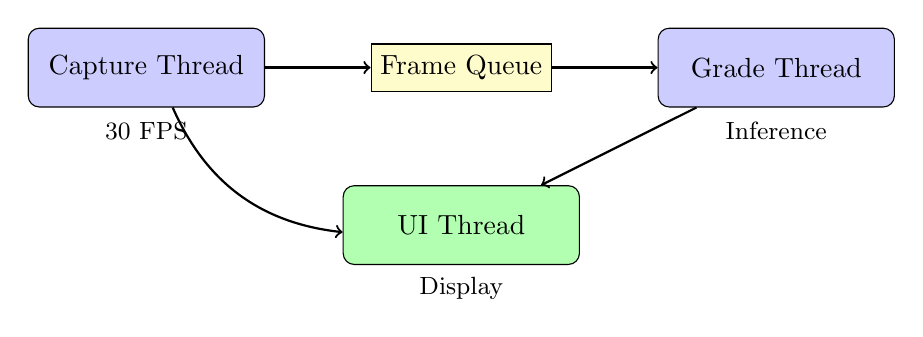
\begin{tikzpicture}[
    thread/.style={rectangle, draw, fill=blue!20, minimum width=3cm, minimum height=1cm, rounded corners},
    queue/.style={rectangle, draw, fill=yellow!20, minimum width=2cm, minimum height=0.6cm},
    arrow/.style={->, thick}
]
    % Capture thread
    \node[thread] (capture) at (0,2) {Capture Thread};
    \node[below of=capture, node distance=0.8cm, font=\small] {30 FPS};
    
    % Queue
    \node[queue] (queue) at (4,2) {Frame Queue};
    
    % Grade thread
    \node[thread] (grade) at (8,2) {Grade Thread};
    \node[below of=grade, node distance=0.8cm, font=\small] {Inference};
    
    % UI thread
    \node[thread, fill=green!30] (ui) at (4,0) {UI Thread};
    \node[below of=ui, node distance=0.8cm, font=\small] {Display};
    
    % Arrows
    \draw[arrow] (capture) -- (queue);
    \draw[arrow] (queue) -- (grade);
    \draw[arrow] (grade) -- (ui);
    \draw[arrow] (capture) to[bend right=30] (ui);
\end{tikzpicture}
\caption{Kiến trúc đa luồng của hệ thống}
\label{fig:threading}
\end{figure}

\begin{itemize}
    \item \textbf{Capture Thread}: Đọc frame từ webcam với tốc độ cao nhất có thể.
    \item \textbf{Grade Thread}: Chạy inference detector + classifier + analyzer.
    \item \textbf{UI Thread}: Hiển thị kết quả, không bị block bởi inference.
    \item \textbf{Frame Queue}: Buffer 1 frame, drop frame cũ nếu inference chậm.
\end{itemize}

\section{Các tham số tối ưu hóa}

Hệ thống cung cấp nhiều tham số điều chỉnh qua biến môi trường:

\begin{table}[H]
\centering
\caption{Các tham số tối ưu hóa hiệu năng}
\label{tab:perf_params}
\begin{tabular}{@{}llp{6cm}@{}}
\toprule
\textbf{Tham số} & \textbf{Mặc định} & \textbf{Mô tả} \\
\midrule
BANANA\_MAX\_FRUITS & 6 & Số quả tối đa xử lý mỗi frame \\
BANANA\_DET\_IMGSZ & 640 & Kích thước input detector \\
BANANA\_CLS\_IMGSZ & 416 & Kích thước input classifier \\
BANANA\_BBOX\_HOLD & 5 & Số frame giữ bbox khi miss \\
BANANA\_ANALYZE\_POLICY & all & Policy chạy analyzer \\
BANANA\_MAX\_INFER\_FPS & 0 & Giới hạn FPS inference (0 = không giới hạn) \\
\bottomrule
\end{tabular}
\end{table}

\section{Tóm tắt chương}

Chương này đã trình bày chi tiết phương pháp thiết kế hệ thống phân loại chất lượng chuối:
\begin{itemize}
    \item \textbf{Kiến trúc 2-stage}: Kết hợp COCO detector (localization) với fine-tuned classifier (classification), tận dụng thế mạnh của từng thành phần.
    \item \textbf{BananaAnalyzer}: Module trích xuất đặc trưng màu sắc (HSV/LAB), hình thái và kết cấu bề mặt.
    \item \textbf{Feature Refinement}: Cơ chế hiệu chỉnh kết quả cho edge cases.
    \item \textbf{Temporal Stabilization}: Xử lý nhấp nháy bbox qua cơ chế hold.
\end{itemize}

\textbf{Từ thiết kế đến hiện thực:} Chương tiếp theo sẽ trình bày quá trình \textbf{cài đặt và triển khai} --- biến các quyết định thiết kế thành mã nguồn hoạt động.

\clearpage
